\documentclass[../Relazione.tex]{subfiles}

\begin{document}

\section{Usabilità su mobile}
	Poiché oggi la maggioranza dell'utenza naviga con dispositivi mobili questa sezione è quasi d'obbligo. 
	In ambito mobile, i problemi di usabilità primari sono l'adattamento della pagina a quest'ambiente (\textbf{mobile responsiveness} ed il suo \textbf{tempo di caricamento} associato (escludendo le specifiche tecniche del dispositivo).

	\subsection{Responsiveness}
		Il layout del sito, purtroppo, \textbf{degrada in maniera non elegante} ed il sito non è ottimizzato per dispositivi mobile; si nota la frattura quasi totale del layout. Il contenuto informativo si adatta bene ma sottoponendo una pagina (in questo esempio la \textbf{Homepage}) al test di ottimizzazione mobile online di Google \href{https://www.google.com/webmasters/tools/mobile-friendly/?hl=it}{Mobile Friendly} fa notare quanto è assente questo supporto.\\Ogni accortezza proposta da Google \textbf{non è implementata.}

		\begin{figure}[!h]
			\centering
			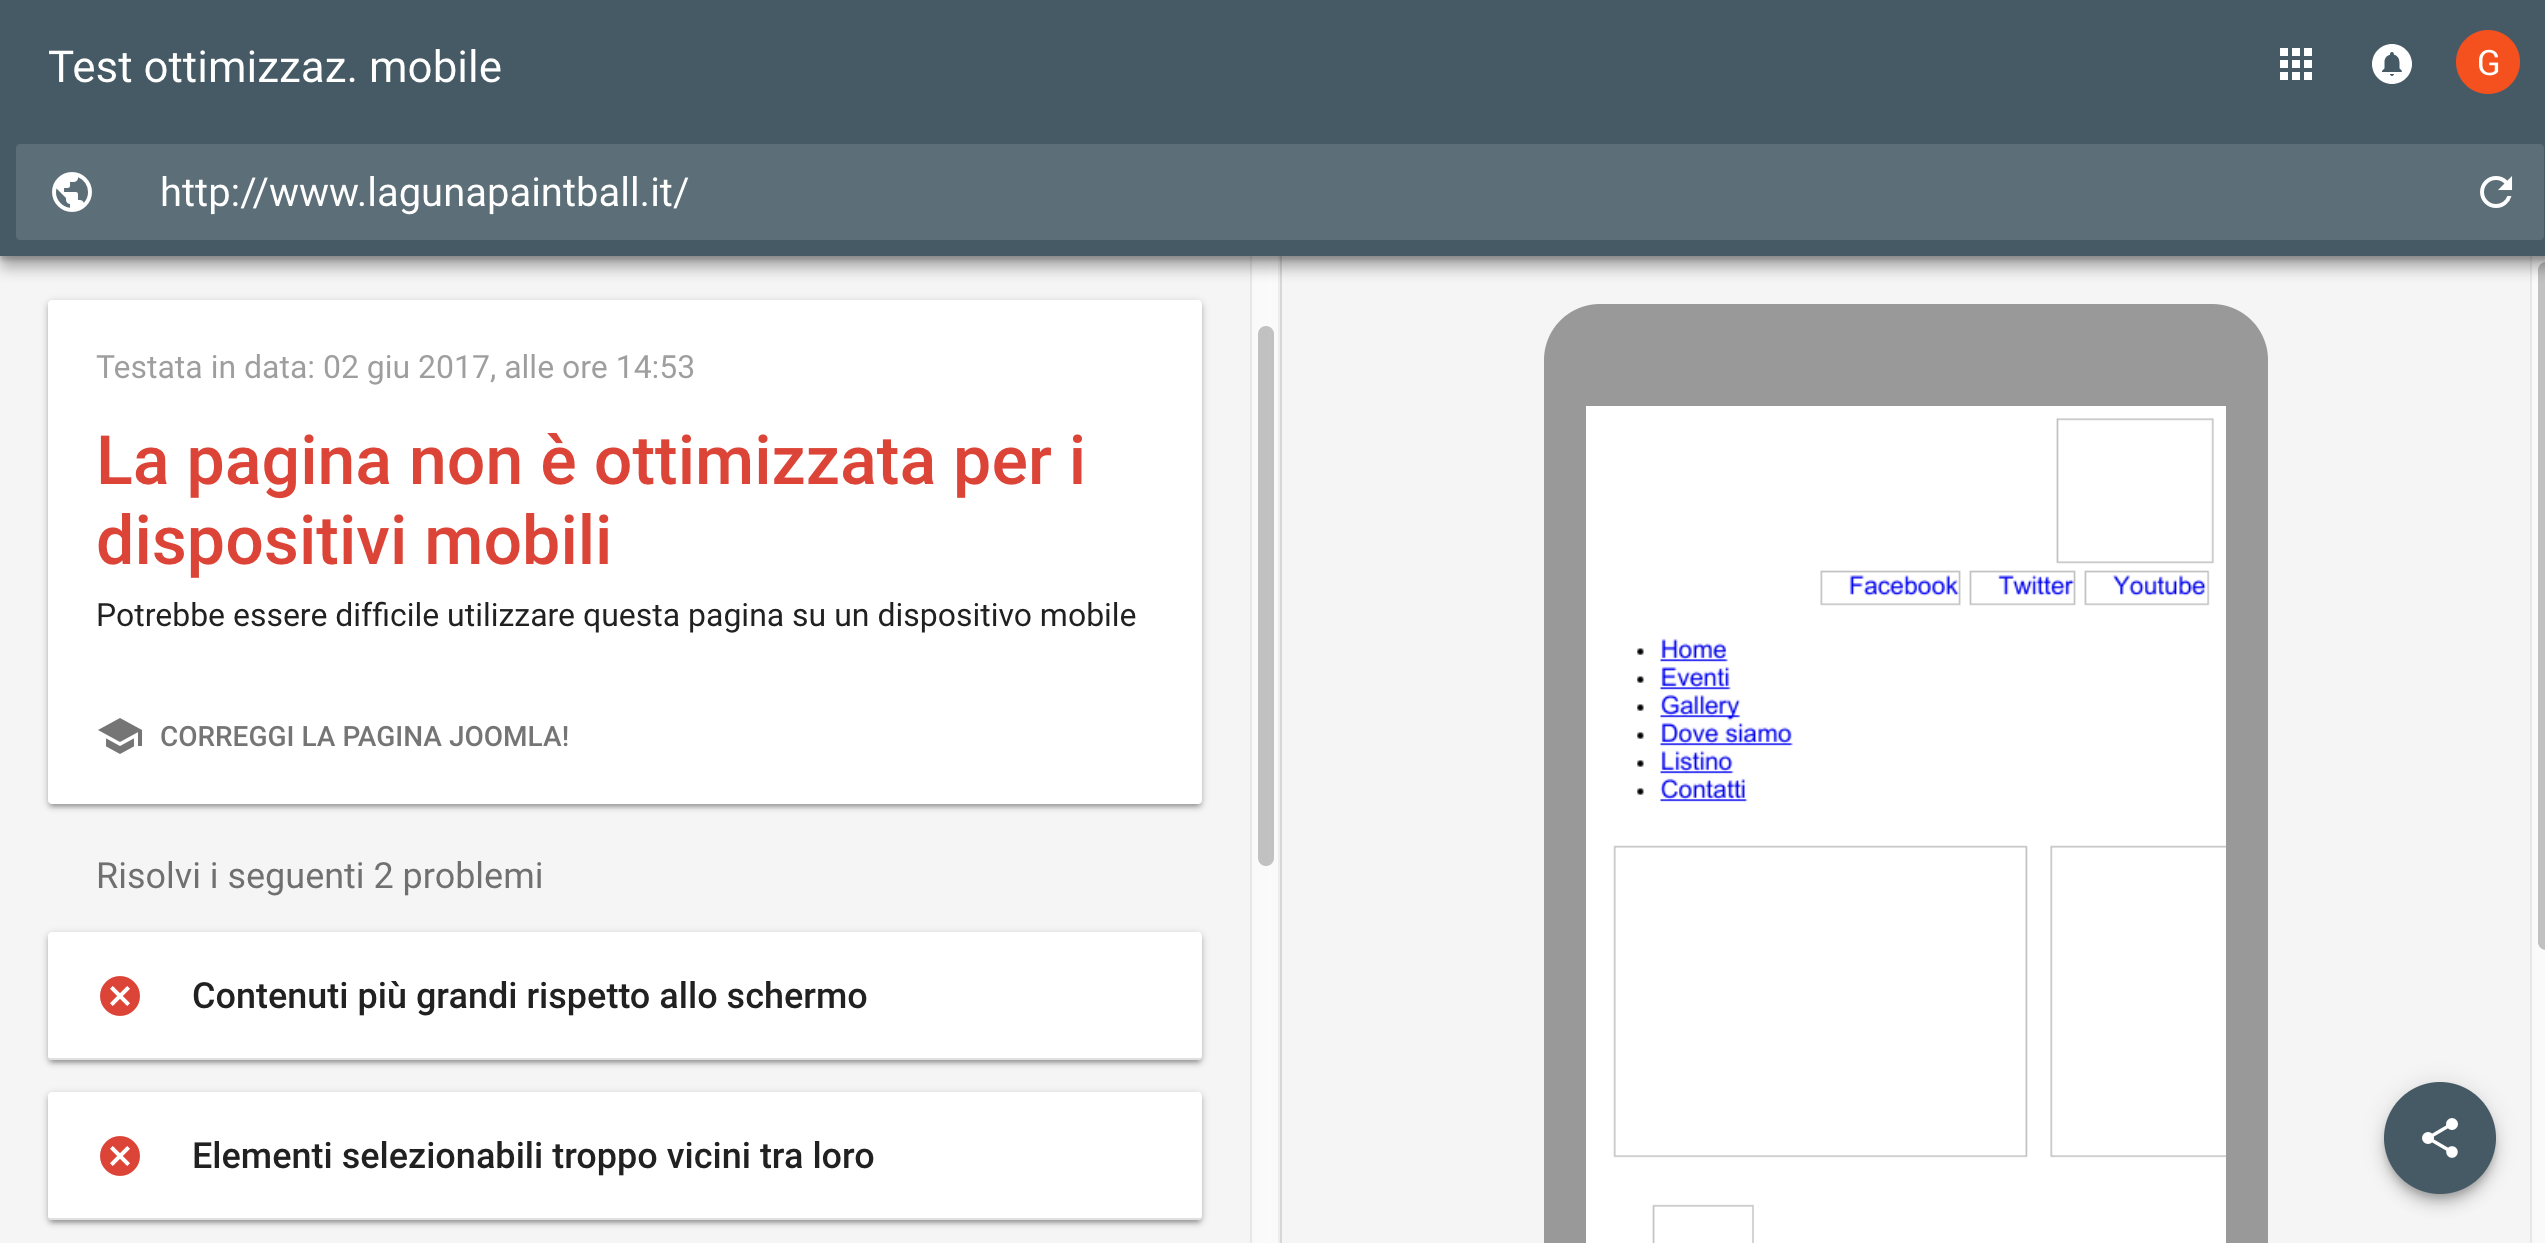
\includegraphics[width=\textwidth]{img/sito/MobileSupport.png}
			\caption{Test ottimizzazione Mobile - I risultati mostrano che la pagina testata non ha il minimo supporto}
			\label{fig:label}
		\end{figure}

\newpage
	\subsection{Tempi di caricamento}
		Molto male anche nei tempi di caricamento; lo strumento \href{https://developers.google.com/speed/pagespeed/insights/}{SpeedTest} di Google assegna un punteggio di \textbf{50 punti su 100} (in ambiente Desktop 60/100).\\
		I tempi di caricamento della sola homepage, usufruendo di una connessione wi-fi con uno smartphone di fascia bassa, misurano più di 5 secondi; ulteriori test con telefoni più prestanti misurano meno di 5 secondi. Ancora un tempo troppo alto se consideriamo che l'utente medio concede al massimo 2 secondi di attesa prima di un cattivo giudizio.
			\begin{figure}[!h]
				\centering
				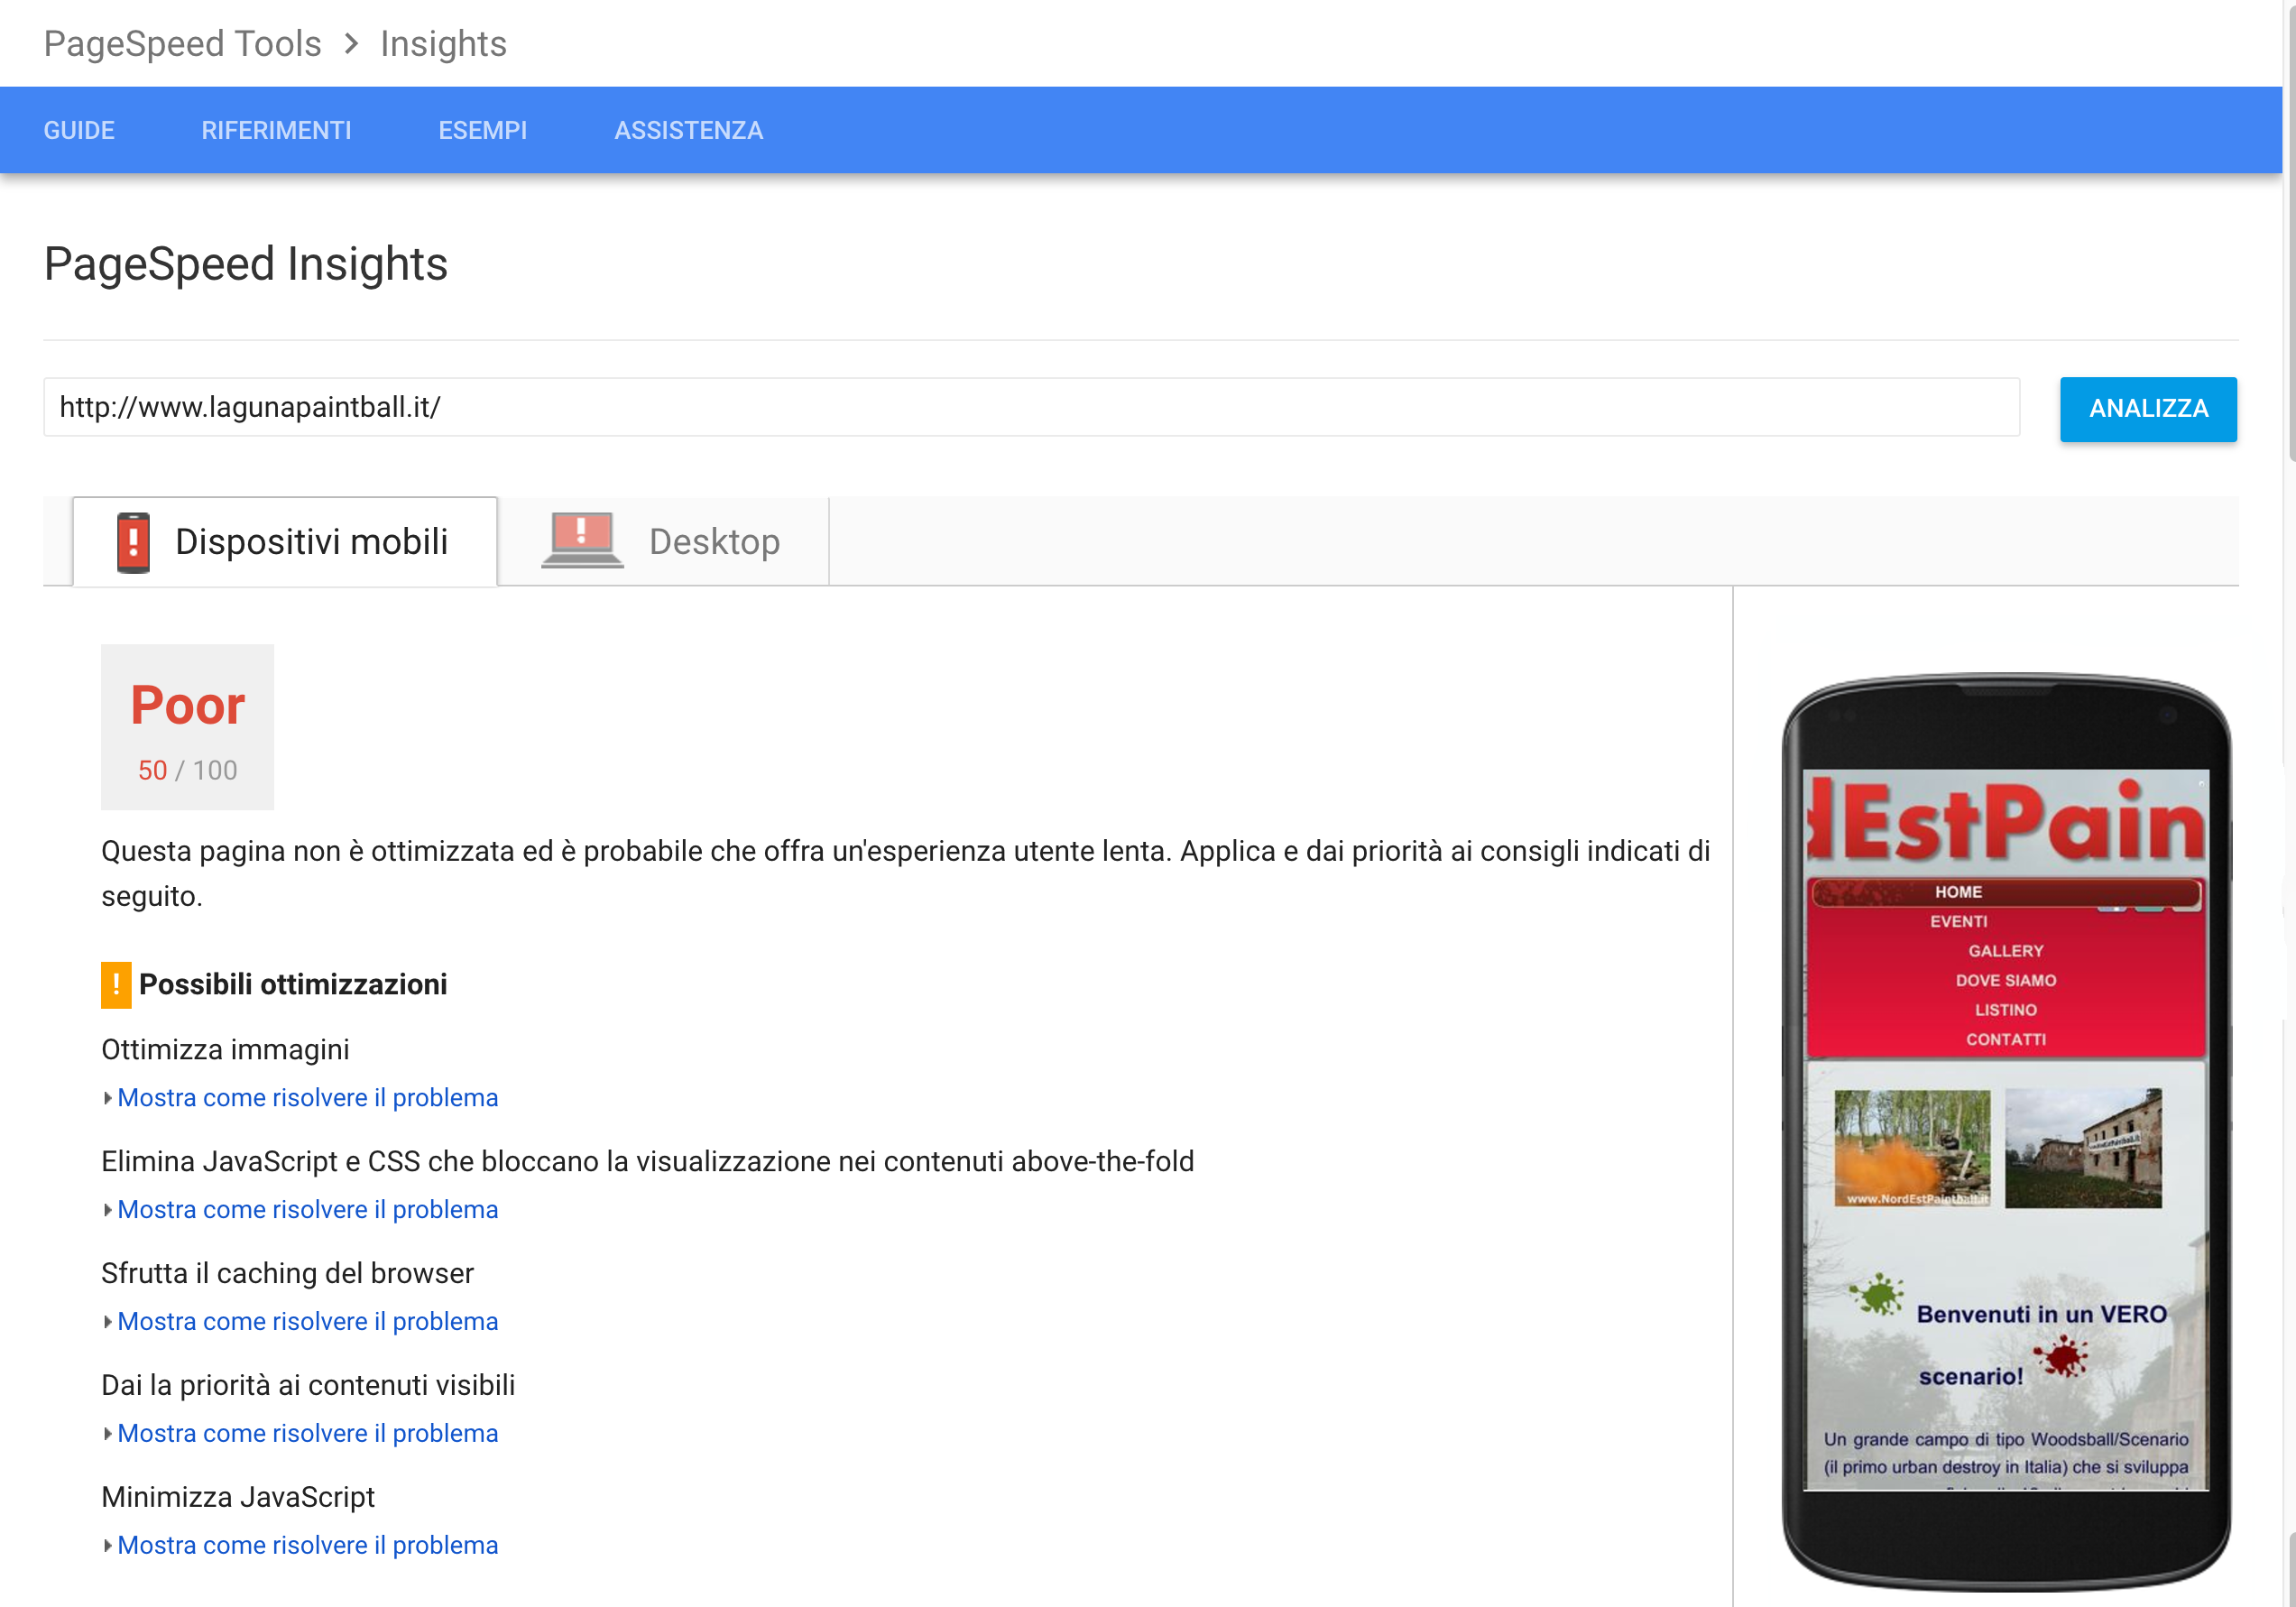
\includegraphics[width=\textwidth]{img/sito/PageSpeedMobile.png}
				\caption{Scarsi risultati evidenziati dallo PageSpeed Mobile}
				\label{fig:label}
			\end{figure}
		Le cause, come suggerisce il pagespeed, provengono da un'errata progettazione che rallenta il caricamento generale:
		\begin{itemize}
			\item \textbf{Contenuti bloccati:} 7 risorse script Javascript e 6 risorse CSS bloccano contenuti above-the-fold, ovvero banner e testo visualizzati in primis per importanza, fondamentali nel decretare il successo o l’insuccesso di una presenza internet, sono bloccati dalla logica di codifica!
			\item \textbf{Il catching} locale del browser non viene sfruttato: una scadenza per le risorse statiche non è impostata;
			\item \textbf{Priorità ai contenuti visibili:} testo e immagini caricate con uguale priorità;
			\item \textbf{Javascript non minimizzato:} compattare il codice JavaScript può far risparmiare parecchi byte di dati e può velocizzare download, analisi e tempo di esecuzione.
		\end{itemize}

\end{document}